\section{\Glsfmtlongpl{rnn}}
\label{sec.rnn}

L'un des principaux défauts que nous avons observés avec les \glspl{mlp} 
et qui nous ont poussés à introduire l'architecture encodeur--décodeur,
est leur incapacité de représenter la dépendance entres les éléments d'une séquence.

Les \glspl{rnn} tentent à résoudre ce problème en introduisant une boucle de rétro-action~\cite{Fathi_2021}.
Cela veut dire que la sortie d'un \gls{rnn} dépend des sorties précédentes aussi bien que de l'entrée.

\begin{figure}[hbt]
    \begin{center}
        \begin{subfigure}{.4\linewidth}
            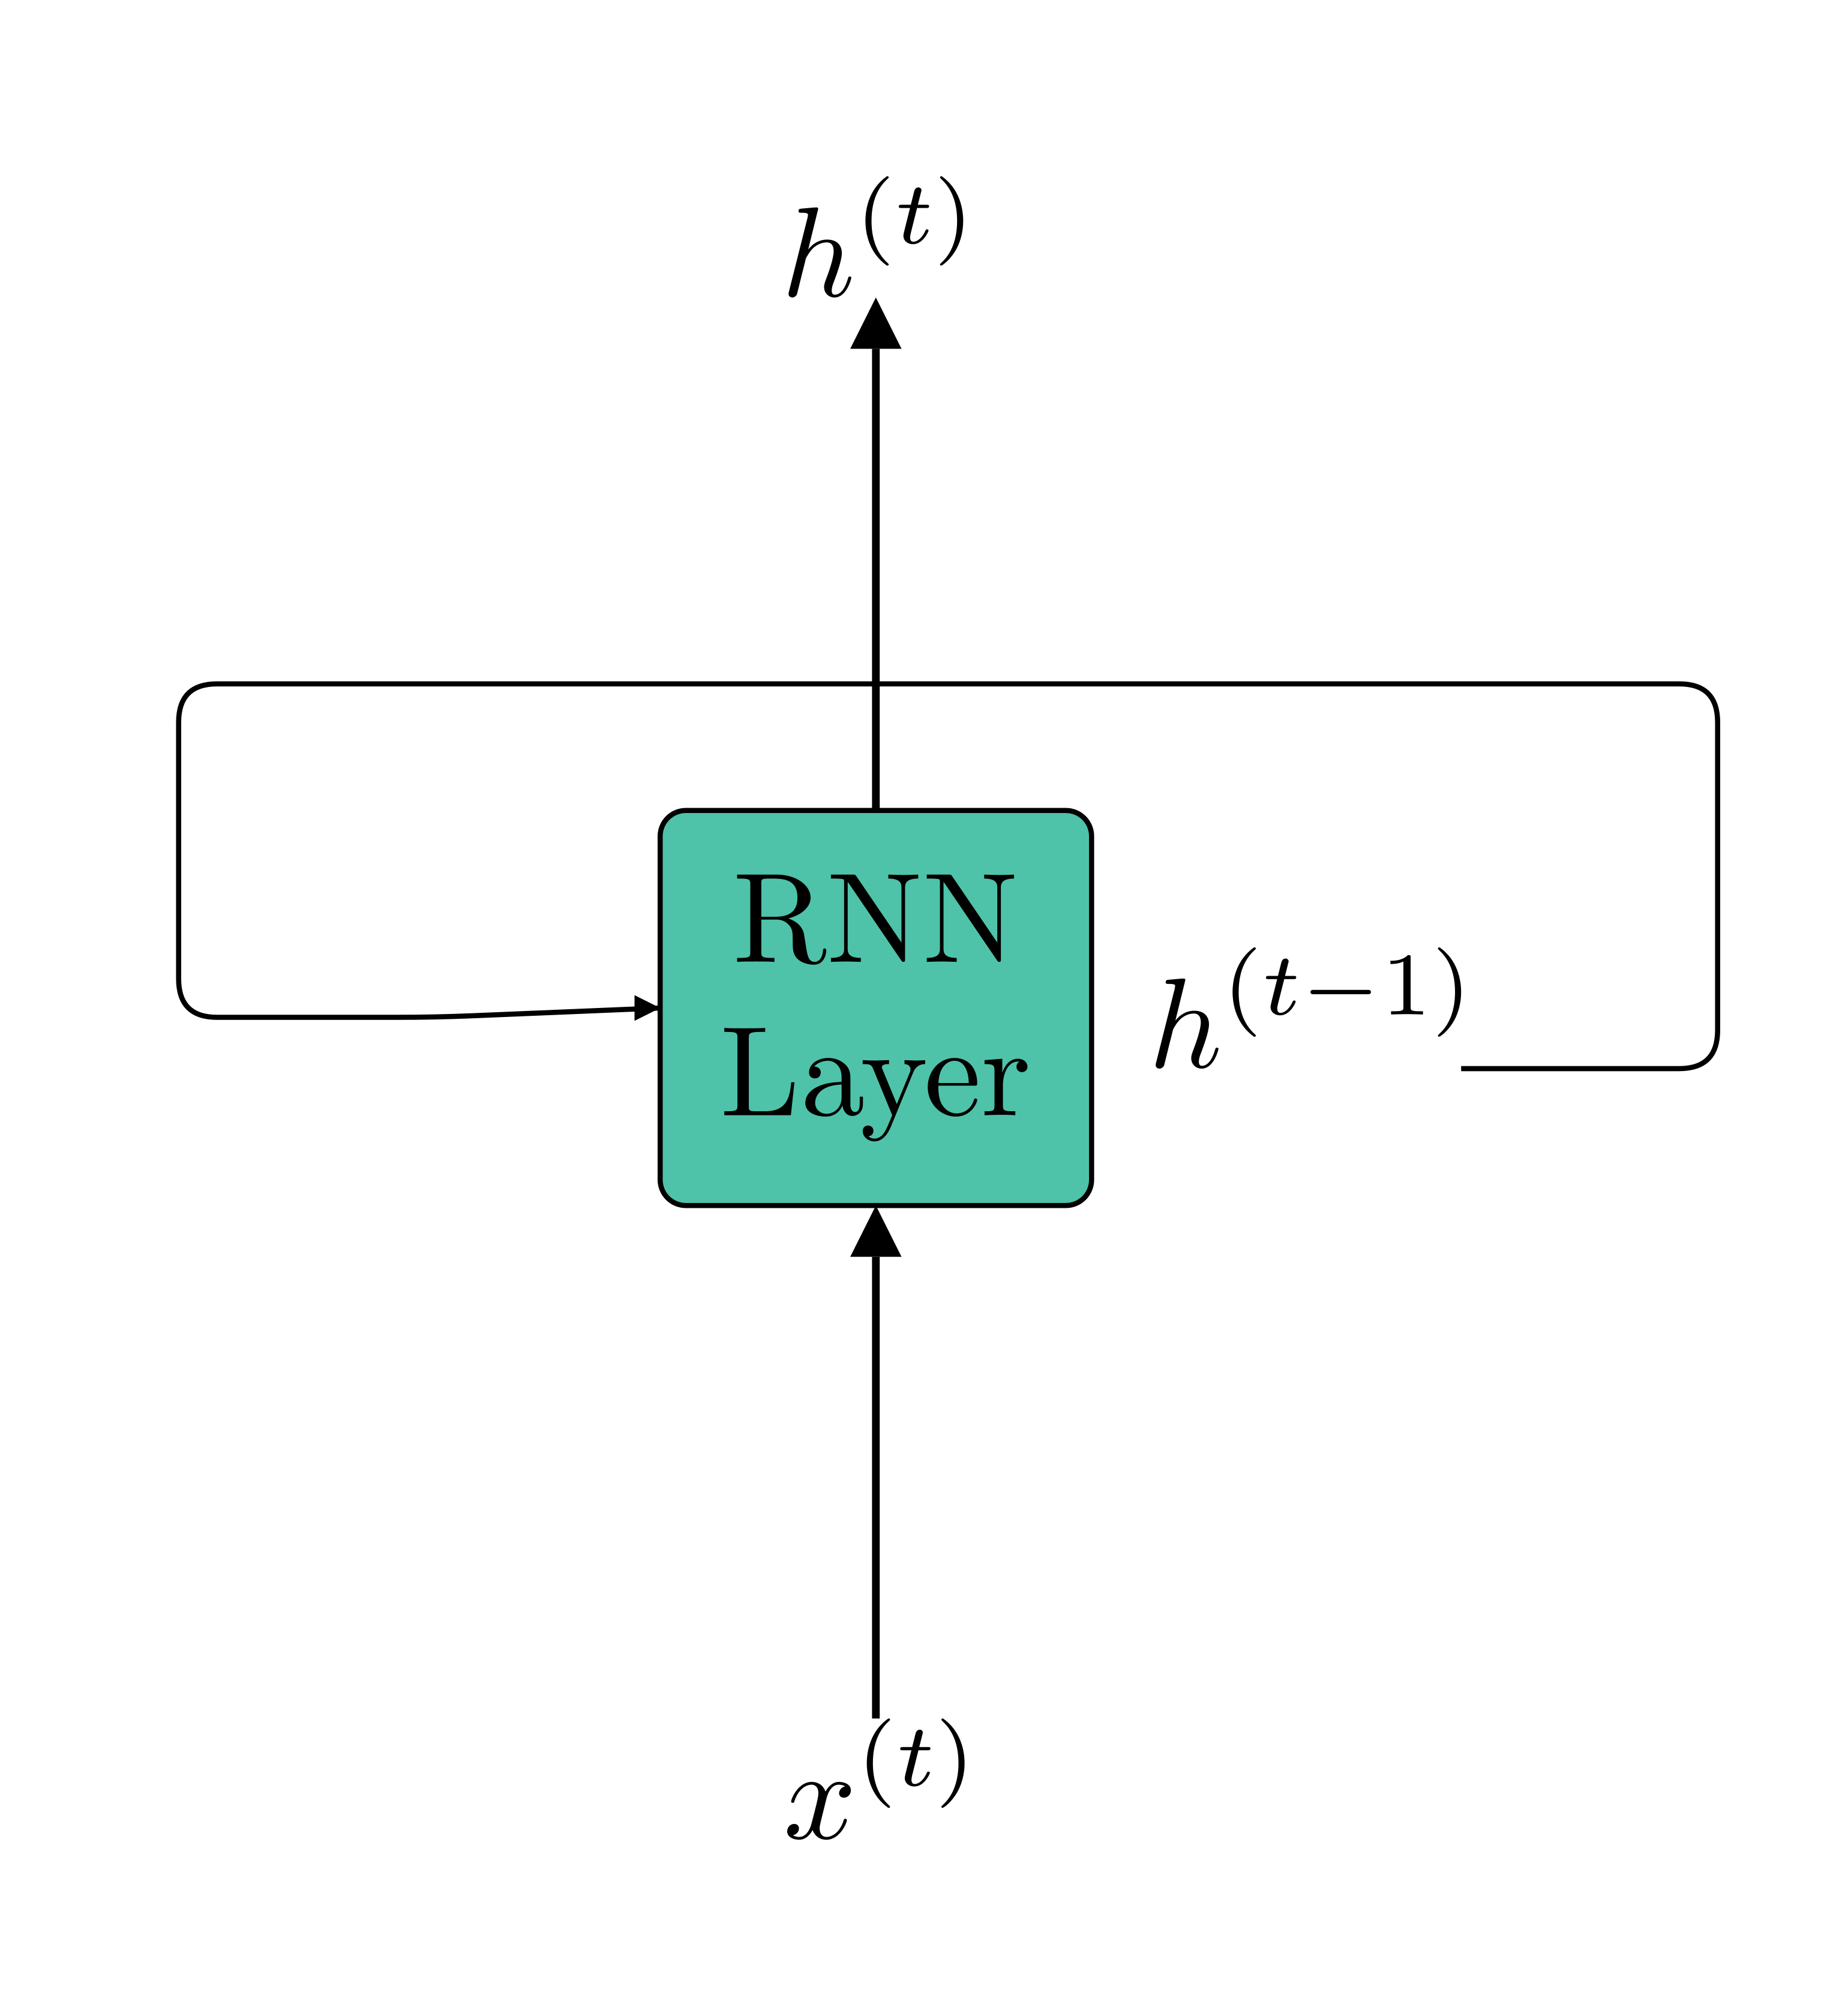
\includegraphics[width=\linewidth]{rnn-loop}
            \caption{Couche récurrente}
            \label{fig.rnn-loop}
        \end{subfigure}
        \begin{subfigure}{.4\linewidth}
            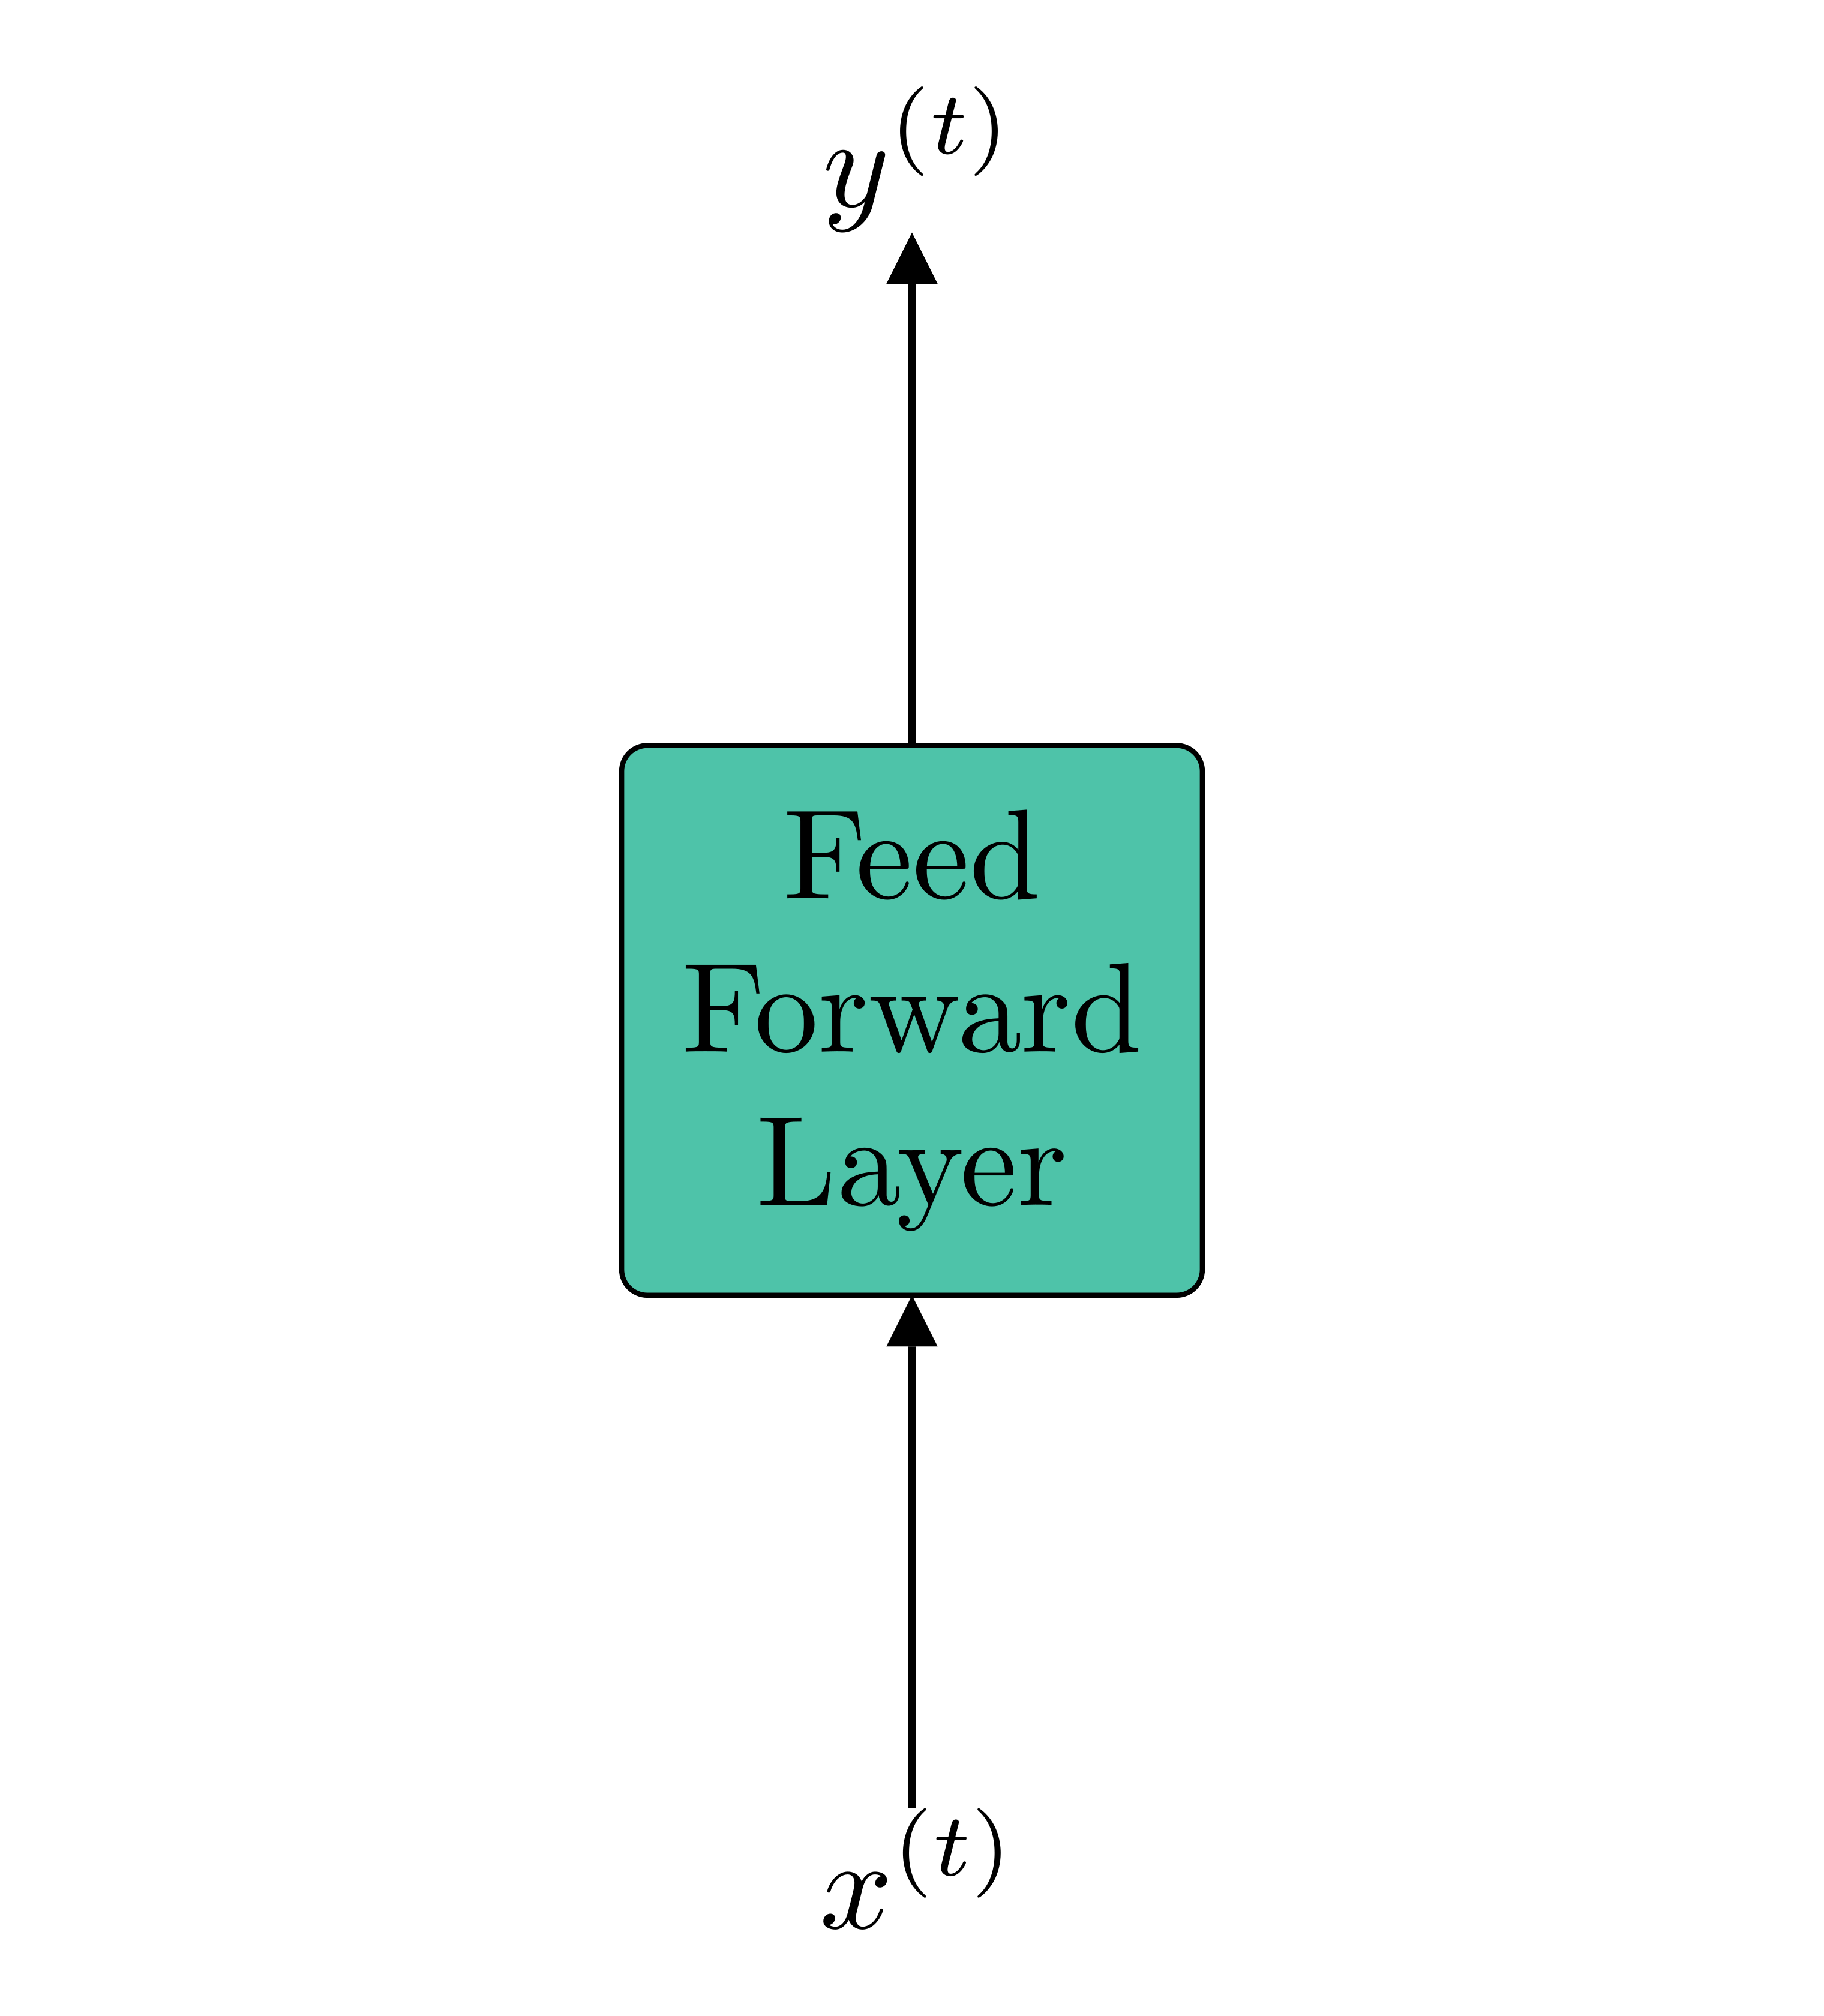
\includegraphics[width=\linewidth]{ffn-layers}
            \caption{Couche feed-forward}
            \label{ffn-layer}
        \end{subfigure}
    \end{center}
    \caption{\glsfmtshort{rnn} v.s \glsfmtshort{ffn}}
\end{figure}

\subimport{}{simple}
